\section{Morphing d'images quelconques}
\label{sec:morphing_images}

\paragraph{} Après avoir abordé la morphose dans des cas simples, notamment celui de formes unies simples et courbes, 
nous allons désormais nous intéresser à la morphose d'images quelconques. De ce fait, l'objectif à atteindre est de pouvoir
passer d'une image à une autre de manière fluide, en conservant les caractéristiques de chacune des images, tout en \important{évitant l'effet juxtaposition}.

\begin{figure}[h!]
    \centering
    \begin{subfigure}{0.4\textwidth}
        \centering
        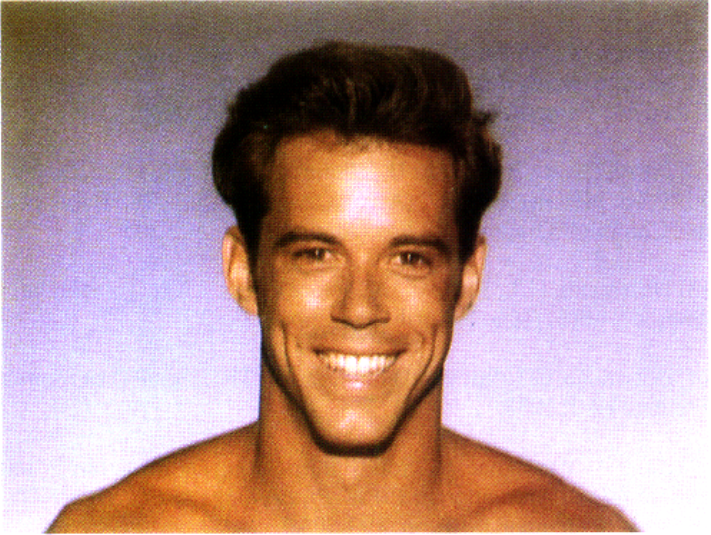
\includegraphics[width=0.8\linewidth]{img/p3/lena.png}
        \caption{Image de départ}
        \label{fig:lena}
    \end{subfigure}
    \begin{subfigure}{0.4\textwidth}
        \centering
        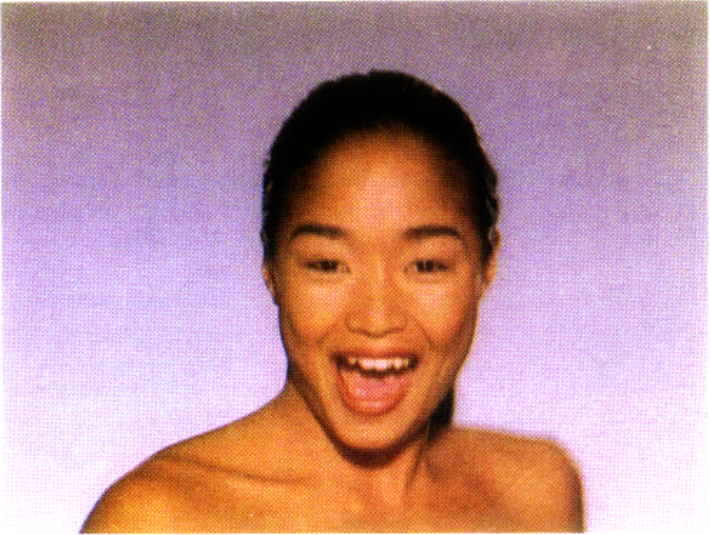
\includegraphics[width=0.8\linewidth]{img/p3/lena2.png}
        \caption{Image d'arrivée}
        \label{fig:lena2}
    \end{subfigure}
    \caption{Paires d'images à morpher \cite{beier1992feature}}
\end{figure}

\paragraph{} Pour ce faire, nous allons nous appuyer sur les travaux de Beier-Nelly \cite{beier1992feature}, qui proposent une méthode de morphing basée sur la paramétrisation de l'image
par des vecteurs de contrôle. Ainsi, chaque pixel de l'image est repéré par une association de positions relatives à ces vecteurs de contrôle. En conséquence de quoi, pour deux images
différentes ayant le même nombre de vecteurs de contrôle, il est possible d'associer chaque pixel de l'une, à un pixel de l'autre (ceci ne signifie pas qu'il existe une bijection entre les pixels des deux images). 

\paragraph{Principe} Le principe de la morphose entre deux images repose sur deux étapes majeures. 
La première consiste à déformer les images de départ et d'arrivée, et la seconde à interpoler les images résultantes.
Ce faisant, il nous est possible d'éviter l'effet de superposition des images. Naturellement, plus le nombre de vecteurs de 
contrôle est élevé, plus la morphose sera précise. De même, un grand nombre d'images intermédiaires permettra d'obtenir
 une animation plus naturelle.

\begin{figure}[h!]
    \centering
    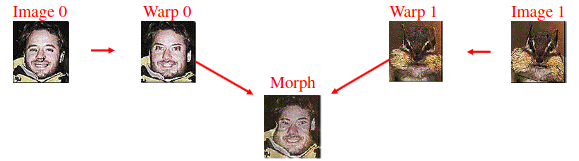
\includegraphics[width=0.8\linewidth]{img/p3/principe.png}
    \caption{Calcul d'un image intermédiaire \cite{CSC320W}}
    \label{fig:morphInter}
\end{figure}

\begin{codeb}
Sur la figure \ref{fig:morphInter}, on peut observer le calcul d'une image intermédiaire \emph{Morph}. 
Explicitement, on a : \couleur{$Morph = (1 - \alpha) \times Wrap_0 + \alpha \times Wrap_1$}, où $\alpha$ est un paramètre variant de 0 à 1.
\end{codeb}

\subsection{Déformation des images}
\label{subsec:deformation}
\subsubsection{Préliminaires}
\begin{definition}
    Soient $P$ une image. On note $w$ sa largeur et $h$ sa hauteur, ainsi que $\mathcal{D}(P)=[0,w]\times[0,h]$.
    On appelle \important{vecteur de contrôle} de $P$ tout couple de points du plan $c=(c_1,c_2)$ tel que $c\in\mathcal{D}(P)$.
\end{definition}

\begin{definition}
    Soient $P$ et $Q$ deux images, ainsi que $p$ et $q$ deux vecteurs de contrôle de respectivement $P$ et $Q$. On définit la
    relation $\sim$ telle que $p \sim Q$ si et seulement si $p$ et $q$ sont appariés. Id est, $p$ et $q$ 
    sont une seule et même entité, mais dans deux contextes (\emph{images}) différents.
\end{definition}
\begin{coder}
    \textbf{Conditions.  } Considérons deux images $P$ et $Q$ à morpher en $N>0$ étapes. 
     Alors, chacune possède $n+1$ vecteurs de contrôle $p_{0},\dots,p_{n}$ et $q_{0},\dots,q_{n}$ tels que pour tout $i \in \{0,\dots,n\}$, $p_{i} \sim q_{i}$.

\end{coder}
\subsubsection{Cas simple: un seul vecteur de contrôle}
\begin{definition}
    Soient $P$ et $Q$ deux images, ainsi que $p$ et $q$ des vecteurs de contrôle de resp. $P$ et $Q$.


\end{definition}
\begin{figure}[h!]
    \centering
    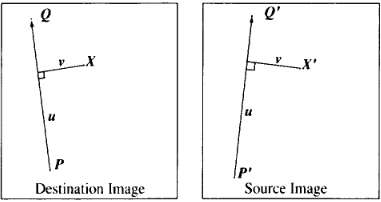
\includegraphics[width=0.8\linewidth]{img/p3/uv.png}
    \caption{Apparaiement à un seul vecteur \cite{beier1992feature}}
    \label{fig:deformation}
\end{figure}